\chapter{Theoretical Framework}
\label{theoframework}




\section{Traffic-related terms}
\subsubsection{Traffic flow}
According to \shortciteA{may1990}, traffic flow studies how travelers interact with infrastructures and with each other, in order to understand the movement of traffic and how can it be improved with less congestion. These travelers include drivers, pedestrians, among others, while infrastructures include roads, signages, stop lights, and other devices that control traffic.

\subsubsection{Traffic speed}
The speed of a vehicle can be computed by measuring the distance it traveled per unit time. Because the speed of each vehicle may be different from its neighboring vehicles, traffic speed is the average of the speed of each vehicle in the given environment. 

\subsubsection{Traffic volume}
Traffic volume refers to the number of vehicles present in a certain road at a given time.

\subsubsection{Traffic density}
Given a length of a road, traffic density is measured by the number of vehicles present. This means that if the traffic density is low, then there is no traffic congestion because the vehicles are apart from each other. In reverse, if the traffic density is high, then the vehicles are close to each other; thus, a traffic congestion.

\subsubsection{Traffic condition}
Traffic conditions refer to the states of traffic at a certain point at a certain time, with respect to traffic flow, speed, volume, and density. It has three major states: light, moderate, and heavy traffic.

\subsection{Traffic Congestion}
Traffic congestion, according to \shortcite{vuchic1994bus}, happens when traffic volume on a particular road goes beyond the road’s capacity. \shortcite{bovy2002congestion} define traffic congestion as the state of traffic flow on a particular road with low speeds and high densities compared to some other state with high speeds and low densities. 

\subsubsection{Road and road segments}
A road is a wide path from one place to another, usually paved for the vehicles to drive on \shortcite{wang2013}. Typically, a road is created for vehicles to head two opposite directions, northbound and southbound. A road segment, on the other hand, is a portion of a road heading in one direction, separated by infrastructures (e.g. train stations, landmarks, intersections).




\section{Weather-related terms}

\subsubsection{Temperature}
Temperature is the measure of the hotness and the coldness of an object. There are three major scales that are being used internationally, \textit{Celsius}, \textit{Fahrenheit}, and \textit{Kelvin}. 

\subsubsection{Dew point}
Dew point is the temperature wherein moisture or \textit{dew} appears on solid surfaces. This is caused by condensation, in which the water vaporizes into its liquid form at certain amounts of pressure. 

\subsubsection{Humidity}
Humidity refers to the quantity of the water vapor contained in the air. Measured in percentage, relative humidity, on the other hand, is the quantity of water vapor in relation to how much the air can hold at a certain temperature. If the air is warm, it has high relative humidity since the air holds more water vapor than cold air. 

\subsubsection{Wind speed}
Wind speed is the average wind speed in the indicated amount of time. Because of the changing temperature, wind speed results from the air going from above average temperature to a lower temperature. 

\subsubsection{Wind Gust}
Wind gust is the short, rapid rise of wind speed before quickly calming. The wind is forced to change its direction and speed quickly because of sudden decrease in temperature,  wind shears, and friction.

\subsubsection{Precipitation}
Precipitation refers to any result of air condensation that falls due to the pull of gravity. This includes, but not limited to, rain, snow, and hail. Usually, precipitation is measured in terms of millimeters (mm).

\subsubsection{Visibility}
Visibility is the measure of how long can we distinguish light or an object at a certain distance.  

\subsubsection{Pressure}
Pressure, also called atmospheric pressure, is the amount of force exerted by the air molecules in a particular surface area of the earth. Meteorologists use millibars (mb) to measure pressure. 

\subsubsection{Cloud Cover}
Cloud cover is defined as the amount of clouds in a fragment of the sky in a particular location. This contributes to the weather condition and visibility. This is usually measured by \textit{okta}.

\subsubsection{Heat Index}
Heat index is the temperature of how hot the human body feels like. This is directly related to air temperature and relative humidity. 

\subsubsection{Feels-like}
Feels-like is the temperature of how cold the human body feels like when the wind touches the skin.




\section{Historical Data}
Historical data is an extensive archive of data that can be utilized to detect regularities or pattern for predicting future outcomes. It ranges from months-worth to years-worth of past data. The following section features sources whose historical data will be used for the research.

\subsection{Traffic Data from MMDA’s Traffic Monitoring System}
The traffic dataset includes traffic conditions for nine major roads in Metro Manila, collected in a 15 minute time interval. The traffic condition can either be \textit{light} (L), \textit{moderate} (M), or \textit{heavy} (H). However, if no information is available, it can also appear as \textit{none} (N).

Major roads from this dataset include EDSA, Commonwealth, Quezon Avenue, España, C5, Ortigas, Marcos Highway, Roxas Boulevard, and SLEX. Each road consists of a number road segments, which includes a northbound lane and a southbound lane. For instance, EDSA consists of 37 road segments (e.g. Balintawak, Kaingin Road, Muñoz).

Table \ref{table:sample_traffic_data} shows a sample raw data collected from MMDA’s traffic monitoring system. From the sample data, it can be observed that despite not having a traffic condition entry, the interval is still being recorded as part of the dataset, having a traffic condition record of \textit{none} (N).

\begin{table}[h]
	\centering
    \footnotesize
	\caption{Sample of Traffic Data from MMDA's Traffic Monitoring System}
	\label{table:sample_traffic_data}
	\begin{tabular}{|l|l|l|p{2.5cm}|p{2.5cm}|}
		\hline
		Date and Time & Road & Segment & Condition (Northbound) & Condition (Southbound) \\ \hline
		2015-01-01 00:00:00 & EDSA & Quezon Ave. & L & L \\ \hline
		2015-01-01 00:00:00 & EDSA & Taft Ave.& M & M  \\ \hline
		2015-01-01 00:00:00 & ESPAÑA & Welcome Rotunda& L & L  \\ \hline
		2015-01-01 00:15:00 & EDSA & Quezon Ave.& N & N  \\ \hline
		2015-01-01 00:15:00 & EDSA & Taft Ave.& M & M  \\ \hline
		2015-01-01 00:15:00 & ESPAÑA & Welcome Rotunda& L & L  \\ \hline
	\end{tabular}
\end{table}


\subsection{Weather Data from World Weather Online}
The weather dataset from World Weather Online includes temperature (in both Celsius and Fahrenheit), humidity (in percentage), pressure (in millibars), wind speed (in both miles per hour and kilometers per hour), and dew point (in both Celsius and Fahrenheit), cloud cover amount (in percentage), heat index (in both Celsius and Fahrenheit), visibility (in kilometers), wind chill temperature (in both Celsius and Fahrenheit), wind gust (in both miles per hour and kilometers per hour), feels-like temperature (in both Celsius and Fahrenheit), and precipitation (in millimeters). This data is sampled every one hour of every day and is a generalized reading for the whole city of Manila.

Table \ref{table:sample_worldweatheronline_weather_data} shows a sample raw data collected from World Weather Online. It could be observed that the conversion of some variables to different units has already been performed as part of the data. Furthermore, missing data is not evident from the samples collected.


\begin{table}[h]
	\centering
	\caption{Sample of Weather Data from World Weather Online}
	\label{table:sample_worldweatheronline_weather_data}
	\begin{tabular}{|l|r|}
		\hline
          Property & Sample Value \\ \hline
          Date & 2015-10-01 \\ \hline
          Time & 0 \\ \hline
          Weather Condition & Moderate or heavy rain shower \\ \hline
          Temperature (\textdegree{}C) & 27 \\ \hline
          Temperature (\textdegree{}F) & 81 \\ \hline
          Wind Speed (m/h) & 2 \\ \hline
          Wind Speed (km/h) & 4 \\ \hline
          Humidity (\%) & 87 \\ \hline
          Visibility (km) & 8 \\ \hline
          Pressure (mb) & 1013 \\ \hline
          Cloud Cover (\%) & 27 \\ \hline
          Heat Index (\textdegree{}C) & 31 \\ \hline
          Heat Index (\textdegree{}F) & 88 \\ \hline
          Dew Point (\textdegree{}C) & 25 \\ \hline
          Dew Point (\textdegree{}F) & 76 \\ \hline
          Wind Chill (\textdegree{}C) & 27 \\ \hline
          Wind Chill (\textdegree{}F) & 81 \\ \hline
          Wind Gust (m/h) & 4 \\ \hline
          Wind Gust (km/h) & 7 \\ \hline
          Feels Like (\textdegree{}C) & 31 \\ \hline
          Feels Like (\textdegree{}F) & 88 \\ \hline
          Precipitation (mm) & 2.8 \\ \hline
	\end{tabular}
\end{table}



\section{Working Day}
A working day refers to a day in which people are assigned on duty in an organization (e.g. company, government, school, etc.) each week \cite{liu2008wdcm}. For most organizations, working day is defined to be from Mondays to Fridays. Non-working days, meanwhile, are from Saturdays to Sundays. As people are on duty during working days, this implies an increase in demand on transportation when going to their respective organizations \shortcite{traffic_trend}. Thus, there is an increase in traffic volume due to the demand during weekdays as compared to weekends.

Aside from weekends, there are also instances in which a weekday can be classified as a non-working day. This occurs during holidays or whenever a public-sector or government announces class or work suspension.



\section{Peak Hour}
A peak hour, or rush hour, is a time of the day where the congestion of traffic in roads or inflation of people in public transports are at its highest peak \shortcite{downs2005still}. There are two peak hours each weekday: the morning peak hour and the afternoon or evening peak hour. These are the times when majority of the people travel and commute to go to work or school. The morning peak hours depict the time when employees and students travel towards their workplace or school, while the evening peak hours suggest the time when they return to their respective homes. These periods may last for more than one hour, and may vary from road to road, city to city, country to country, and seasonally. 
\section{Extreme Weather Disruptions}
Extreme weather disruptions such as typhoons and low-pressure areas have brought heavy and prolonged precipitation which often causes flooding in some areas. One example of these extreme weather disruptions is Typhoon Goring that occurred from July 22, 2015 until July 26, 2015. Weather disruptions typically produce a significant amount of precipitation in just one day. These prolonged rain periods usually last for days, thus building up the effects it brings as time goes by.





\section{Traffic Model}
% definition of traffic model
Mathematically, a traffic model is a representation of traffic in the real-world \shortcite{mahmud2016}. These models exist to help researchers understand how traffic works and how can the congestions be minimized by simulating them in a way that researchers can explore and manipulate. 

% macroscopic and microscopic model
There are two major types of traffic modeling: \textit{macroscopic} and \textit{microscopic} \shortcite{mahmud2016}. A macroscopic traffic model deals with the properties of transportation elements in the bigger picture. This includes the study of traffic flow, density, speed, volume, among others. A microscopic traffic model, on the other hand, deals with characteristics of the individual transportation elements. This covers driver behavior, how the vehicles move, among others. 




\section{Linear Interpolation}
Using surrounding data points, interpolation can be used to determine the value of an unknown point in a line. Linear interpolation is one method of interpolation where it assumes a linear or straight line relationship between two known points. It is used to approximate value through the weighted average of two points.




\section{Correlation}
% Spearman’s rank correlation coefficient
The Spearman's rank correlation coefficient is an approach for statistical dependence between two independent variables while not consider the parameters of a frequency distribution (nonparametric) \shortcite{Zar1972SignificanceCoefficient, Liu2010ARecognition, Gauthier2001DetectingCoefficient}. The rank correlation coefficient, $r_s$, can be expressed using a monotonic function as: 

\begin {equation}
r_s = 1 - \frac{6 \sum a^2}{N(N^2 - 1)}
\end{equation}

\noindent where $r_s$  represents the Spearman’s rank correlation coefficient, $a$ denotes the ranked difference between the $i$th measurements for the two random variables, and $N$ is the number of measurements in each of the two random variables in the correlation \shortcite{Zar1972SignificanceCoefficient}. Spearman’s $r_s$ measures the strength and course of the \textit{monotonic} relationship between ranked variables. \shortciteA{Hauke2011ComparisonData}, meanwhile, explain that Spearman’s $r_s$ can be considered as the correlation coefficient of Pearson that deals with ranks.  

% Pearson’s product moment correlation coefficient
Pearson’s product moment correlation coefficient, commonly Pearson’s correlation coefficient or Pearson’s r, is the most commonly used correlation statistic to measure the strength and course of the \textit{linear} relationship between two continuous variables \shortcite{ahlgren2003}. It is expressed using this function:

\begin {equation}
r = \frac{\sum (A - \bar{A})(B - \bar{B})}{\sqrt[]{\sum (A - \bar{A})^2 \sum(B - \bar{B})^2}}
\end{equation}

\noindent where $r$ represents the Pearson’s r, $A$ and $B$ denote the two variables being observed, and $\bar{A}$ and $\bar{B}$ are the averages of the two variables respectively. 

% Results of Pearson and Spearman
Both correlation analysis outputs a value between -1 to +1. If the result of a correlation is close to +1, then variable A has a positive relationship with variable B; vice versa, if the result is close to -1, then variable A has a negative relationship with variable B. If the result is approaching 0, then variable A has no relationship with variable B. Table \ref{table:correlation-results} shows the correlation relationships with their corresponding ranges, where $x$ is the exact correlation result. 


\begin{table}[h]
\centering
\caption{Results of Pearson and Spearman}
\label{table:correlation-results}
\begin{tabular}{|l|r|}
\hline
Correlation Relationship         & \multicolumn{1}{l|}{Value}        \\ \hline
very strong positive correlation & 0.9 $<$ x $\leq$ 1.0   \\ \hline
strong positive correlation      & 0.7 $<$ x $\leq$ 0.9   \\ \hline
moderate positive correlation    & 0.5 $<$ x $\leq$ 0.9   \\ \hline
low positive correlation         & 0.3 $<$ x $\leq$ 0.5   \\ \hline
no correlation                   & -0.3 $<$ x $\leq$ 0.3  \\ \hline
low negative correlation         & -0.5 $<$ x $\leq$ -0.3 \\ \hline
moderate negative correlation    & -0.7 $<$ x $\leq$ -0.5 \\ \hline
strong negative correlation      & -0.9 $<$ x $\leq$ -0.7 \\ \hline
very strong positive correlation & -1.0 $<$ x $\leq$ -0.9 \\ \hline
\end{tabular}
\end{table}

% Advantage of Spearman over Pearson
Although Spearman is considered a Pearson’s r measure in terms of ranks, there are advantages that enable Spearman to be a more powerful measurement over Pearson \shortcite{Gauthier2001DetectingCoefficient}. Spearman’s rank correlation coefficient is not affected by the distribution of the values, unlike Pearson’s r, which normal distribution is analyzed. Furthermore, instead of the raw data, it does not care for outliers because it deals with the ranks of the data. In addition, the data does not need to be in time-series, where the intervals are regular. In contrast, since Spearman disregards the outliers when it turns the data into ranks, there is a loss of information. Moreover, it is less powerful than the Pearson’s r if the data is normally distributed.

\subsubsection{Autocorrelation}
Autocorrelation, sometimes called \textit{serial correlation} or \textit{lagged correlation}, is defined as the correlation of a time series to itself. The series of numbers arranged in time is correlated to the values of its own past and future. The purpose of autocorrelation is to find out if there is a pattern repeating in the data. The formula for autocorrelation is as follows: 

\begin{equation}
r_{k} = \frac{\sum_{i=1}^{N-k}(X_{i} - \bar{X})(X_{i+k} - \bar{X})} {\sum_{i=1}^{N}(X_{i} - \bar{X})^{2} }
\end{equation}

\noindent where $k$ denotes the lags and $N$ as the number of observations in the series.




\section{Feature Engineering}
Feature engineering is important for any system that uses machine learning. The performance of machine learning algorithms depends on how the data was presented to them. If they accept raw data directly, they would not give the intended results since machine learning algorithms do not have the capacity to extract insightful features from raw data automatically. This is where feature engineering comes in. It is using the domain knowledge of and from the raw data and create insightful features which would help machine learning algorithms to perform better. 

A feature is a property that is common with all the independent units in the raw data. Choosing the right features for the model is of utmost necessity. To yield better results, models should be simple and be more flexible, which better features would produce.

The process of feature engineering is difficult and exhaustive. At first, a lot of features need to be decided and created regardless of its relevance. Afterwards, these features would be checked with the model to identify how and which features would help the model. Then, to avoid overfitting, feature selection should be used. This process would repeat until certain features are finalized and used with the model.





\section{Fusion Techniques}
To achieve the best performance, fusion techniques were made for designing systems which recognize patterns. By combining data, features, or decisions from a set of sensors, better inferences are made and accuracy is improved \shortcite{sohn2003}. Fusion techniques are applied in the field of military, where targets are automatically recognized \shortcite{bosse2006}, in the field of image processing for medicine \shortcite{constantinidis2001}, face recognition \shortcite{mangai2010}, robotics \shortcite{jimenez1999}, among others. There are three levels for fusion techniques: \textit{data fusion, feature fusion, } and \textit{decision fusion}. In this paper, only the feature fusion and decision fusion will be discussed. In addition, there are numerous techniques to solve fusion problems, but in this paper, only neural networks and weighted average will be discussed.

\subsection{Fusion Levels}
\subsubsection{Feature Fusion}
Features are the most essential information needed to accomplish any classification task. Although important, not all features contribute to the performance of a classifier. Features that do not match the rest of the dataset can have an effect to the pattern recognized by the classifier. Thus, they should be removed from the dataset \shortcite{mangai2010}. The process of improving or obtaining new features is called feature fusion \shortcite{castanedo2013}. 

\shortciteA{Dasarathy1997SensorApplications} broke down the common hierarchy of fusion into five levels. In the said breakdown, he defined feature fusion as the Feature In- Feature Out Fusion (FEI-FEO). This fusion process accepts and outputs features. Feature fusion can be divided into three methods:  feature ranking and selection, feature extraction, and combination \shortcite{mangai2010}.

\shortciteA{mangai2010} described feature ranking and selection as the soul of feature fusion. It aims to find the optimal subset that can represent the entire dataset. In feature extraction, on the other hand, features are reduced and ranked for a better analysis \shortciteA{Dasarathy1997SensorApplications}. Lastly, feature combination derives new features from at least two selected features.

Another fusion level that accepts features is the Feature In-Decision Out Fusion (FEI-DEO). Its difference with the FEI-FEO Fusion is that instead of having features as its output, it outputs a decision instead. Some researchers refer to this as either feature fusion because of its input or decision fusion because it outputs a decision. It all depends on the researcher’s view  \shortcite{Dasarathy1997SensorApplications}. It is commonly used by researchers for pattern recognition systems that generates a decision based on inputs from different sensors \shortcite{castanedo2013}.

With the issues involving the validity of decision fusion for the affective field, \shortciteA{dmello_graesser_2010} used feature fusion for a multimodal affect detection system. The researchers combined features to generate a better distinction between common human experiences such as confusion, frustration, engagement, delight, boredom, and neutral. They concatenated features from three sensory channels to produce a multichannel feature set. As a result, they were able to generate four multichannel models: Facial-Dialogue (FD) model, Facial-Posture (FP) model, Dialogue-Posture (DP) model, and Facial-Dialogue-Posture (FDP) model. They used feature selection to filter out a number of features that have the highest F-ratio. These features were then combined with the set of features selected from the other channel. 

\shortciteA{geetha_radhakrishnan_2013} were able to get satisfactory classification results after fusing fingerprint and palmprint features for a multimodal biometric authentication system. It aims to identify the set of most important features that can be used for a better recognition accuracy.The researchers claimed that fusing the features extracted from 2D Gabon  filter, stationary wavelet transform (SWT), and principal component analysis (PCA) by concatenation would result into a large feature set. This makes computing match scores more laborious. Hence, they used a wavelet-based fusion algorithm to fuse the extracted features. After using SWT to extract line information, the researchers used the mean-max fusion method to fuse the said features.

\subsubsection{Decision Fusion}
% definition
A decision is a conclusion stemmed from facts of a discerned events and activities \shortcite{castanedo2013}. As the high-level fusion technique, the decision fusion is more complicated since it inputs decisions from multiple classifiers to obtain one accurate decision \shortcite{mangai2010}. \shortciteA{Dasarathy1997SensorApplications} defines decision fusion as the Decision In - Decision Out (DEI-DEO) fusion in his five-step hierarchy of fusion based on input and outputs (see \figref{fig:dei-deo}). This combines multiple decisions from the input and outputs a more appropriate decision.


\begin{figure}[h]
	\centering
	\captionsetup{justification=centering}
	\scalebox{.50}{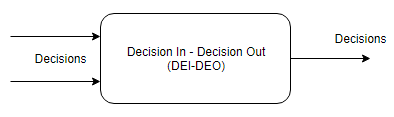
\includegraphics{dei_deo.PNG}}
	\caption{Dasarathy’s Decision In - Decision Out (DEI-DEO)}
	\label{fig:dei-deo}
\end{figure}

%advantages
\shortciteA{Dasarathy1997SensorApplications} also argues that while DEI-DEO fusion does not always trump data or feature fusion, the whole system does not fail if one of the sensors fail, unlike the other fusion techniques. He further explains that the DEI-DEO has less computational demands than the data or feature fusion, and that the bandwidth for communication is not important.

\shortciteA{castanedo2013} states one of the most used methods for decision fusion. The first method is the \textit{Bayesian Method}. This technique combines facts from probability theory rules, where the input and the outputs are probabilities in between [0, 1]. This method is derived from the Bayes rule: 

\begin{equation}
P(B | A) = \frac{P(A | B) P(B)}{P(A)},
\end{equation}

\noindent which gives us the probability of $B$ given $A$. However, because the probabilities $P(A | B)$ and $P(A)$ are not always known, it may not be applicable to some cases. Furthermore, \shortciteA{hall2001} state that the Bayesian method has a complexity problem if there are more than one possible result for $P(B | A)$. 

% applications
Other than Bayesian method, there are other techniques that can be applied to decision fusion, such as the Dempster-Shafer inference, abductive reasoning, semantic methods \shortcite{castanedo2013}, logistic function, weighted decision methods \shortcite{sohn2003}, projection pursuit, majority voting, fuzzy logic, and neural networks \shortcite{jimenez1999}. 


\subsection{Fusion Algorithms}
\subsubsection {Neural Networks}
One of the techniques that can solve fusion problems is through neural networks \shortcite{fincher1990}. The advantage of having neural network as a technique for fusion over statistical approaches, such as Bayesian Method, is that it does not need to know certain probability errors beforehand. It can train itself with the current facts at hand and still get accurate results.  In the following papers, they used neural networks to fuse multiple sensors by recognizing the patterns given the inputs via their supervised training algorithm such as perceptron and backpropagation.
 
\begin{figure}[h]
	\centering
	\captionsetup{justification=centering}
	\scalebox{.6}{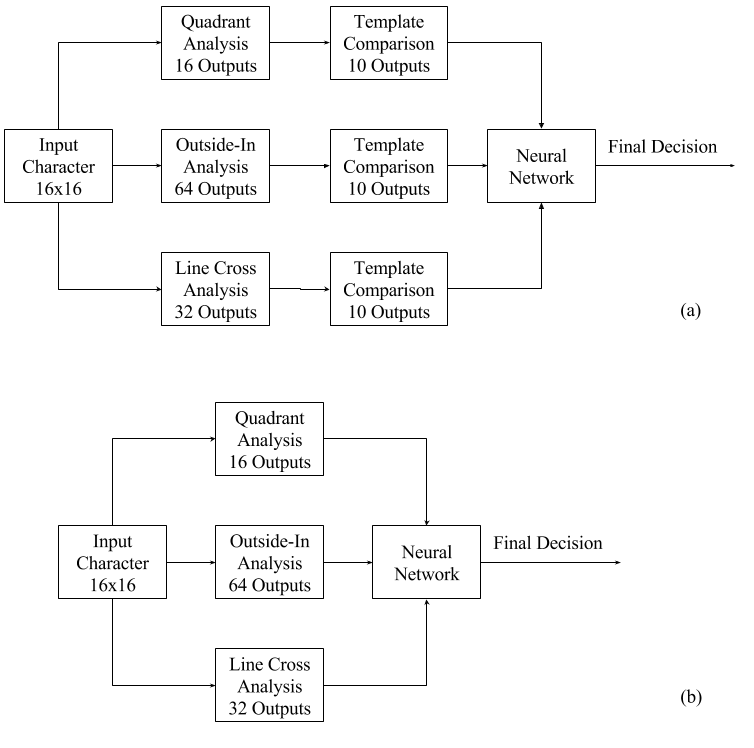
\includegraphics{fincher_approach.png}}
	\caption{(a) Structure of the Fincher’s Pre-Detection Approach, and (b) Structure of the Fincher’s Post Detection Approach}
	\label{fig:fincher_approach}
\end{figure}

In \shortciteA{fincher1990}, they used neural network-based data fusion for recognizing patterns between handwritten and computer-made numbers. The network is fed a 16 $\times$ 16 input character, and outputs the number recognized. They used two approaches in fusion: pre-detection and post-detection. In pre-detection, the input is fed into three algorithms: Quadrant Analysis, Outside-In Procedure, Line Cross Analysis. The outputs of these three algorithms are then compared to a template and creates decisions based from the algorithm outputs. These decisions are then fused through a neural network. In post-detection the outputs of the three algorithms are fed straight to the neural network to avoid loss of data. In this paper, pre-detection detected the correct pattern 93\% of the time than post-detection which detected the pattern 86\% of the time. The network bases its decision on the aspects of the input such as how close is one pixel to the other, and the importance of a value in a pixel. The network was trained through a supervised learning algorithm to merge and recognize the patterns based from the features of the input. The pre-detection follows the DEI-DEO fusion where the decision of the template comparisons are fused to generate the final decision, the pattern recognized from the inputs. On the other hand, the post-detection follows the FEI-DEO fusion where the input of the network is the features of the 16 x 16 input character and the output is the pattern recognized from the input. \figref{fig:fincher_approach} illustrates the pre-detection and post-detection approach.

Likewise, in \shortciteA{dai1999}, they used neural networks for image processing to recognize changes between pictures of the same location of different times. The network is fed raw data from multiple sensors sequentially into 12 input layer units. Like \shortcite{fincher1990}, the network bases its decision from the inputs given. Additionally, the network’s hidden units play the role as the change extractor - one that can recognize and extract changes of the input and pass it to the next hidden layer. Finally, the network will output change map. 

In \shortcite{jimenez1999}, they compared different methods of decision fusion (DEI-DEO), including multilayer neural networks, in hyperspectral imaging. In their architecture, the inputs for their neural network are the decision outputs from different classifiers, whose inputs are vectors of a spectral band in an image. The network was trained through Perceptron supervised training algorithm. Merging the inputs via supervised learning, their output is a single decision obtained from the training of the neural network, identifying the object in the image. 

\subsubsection{Weighted Average}
The Weighted Average is a signal-level fusion method that takes the weighted average of repeating information from the original inputs \shortcite{king2017, yan2011, meurant1992}. \shortciteA{king2017} claimed that using this method will ease the effect of unwanted data in the final estimation. This method can be used to estimate user activity details such as intensity, postures, and fundamental static for activity recognition systems. 

\shortciteA{yan2011} proposed the use of the weighted average method on ships traffic flow data. They used data fusion to produce a higher estimation accuracy from multiple sensors. The researchers multiplied the number of ships with its corresponding weight then obtained the average of the produced weighted inputs. They then applied a distribution method to the original data to eliminate the unwanted data. 



\section{Neural Networks}
%ARTIFICIAL NEURAL NETOWKR
\subsection{Artificial Neural Network}
Inspired from the nonlinear characteristics of Biological Brain System, the work performance of artificial neural networks (ANNs) can be compared to the workings of the human brain system \shortcite{ANN:2016}. While handling uncertainty and non-linearity at the same time, ANNs provide “intelligent processing functions” in order to predict, learn, and memorize \shortcite{sommer2013}. 
ANN can be applied to every situation where the input variables have a relationship with the output variables. The network for ANN consists of 3 layers in order, the input layer, hidden layer and output layer. Each layer consists of 1 or more units or neurons. 
\begin{figure}[h]
	\centering
	\captionsetup{justification=centering}
	\scalebox{.8}{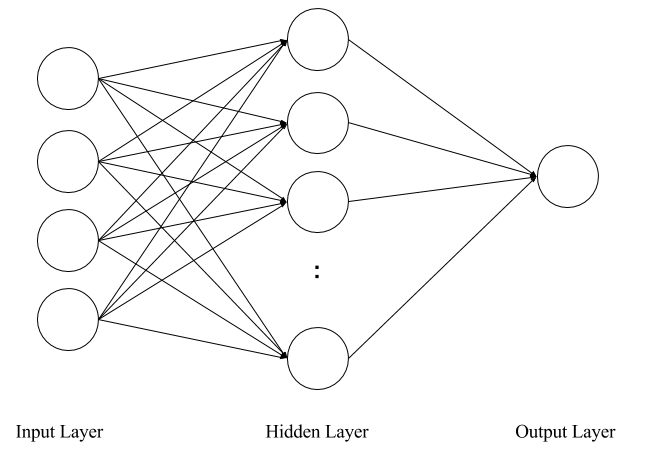
\includegraphics{Network_graph_of_a_One-Hidden_layer_ANN.png}}
	\caption{Network graph of a One-Hidden layer ANN}
	\label{fig:annexample}
\end{figure}

\figref{fig:annexample} shows a the network graph of a One-Hidden layer ANN. Each set of inputs is modified by unique weights in unit connections, and biases in unit. Training in ANN involves adjusting all the weights and biases to have the correct output. A conventional ANN uses backpropagation for its training algorithm \shortcite{Hamad2017}. Backpropagation is a training algorithm which trains the neural network from the input layer to the output layer initializing the weights and biases, and then propagate back from the output layer to the input layer to adjust the weights and biases from the differences between the generated output to the expected output. In backpropagation, each unit that receives a value gets adjusted using an activation function. This training process is repeated a number of times until training error is close to optimal, or until the network reaches the maximum number of epochs. Once backpropagation is finished, the network is trained. The weights ($w$) are adjusted by many learning algorithms such as the Error Correction Learning where the connection weigths between unit $i$ and unit $j$ are adjusted in terms of the difference between the desired and the computed value. A multilayer error correction weight adjustment formula is defined as 
\begin{equation}
w_{ij}^{new} = w_{ij}^{old} - \eta \frac{\partial  E}{\partial  w_{ij}^{old}}
\end{equation}
\noindent where $\eta$ is the learning rate - the percentage the network minimizes the error rate in each iteration and $E$ is the square of errors of the desired output and actual output which can be defined as 
\begin{equation}
E = \frac{1}{2} \sum_{j=1} \left(b_{j} - z_j\right)^2
\end{equation}
\noindent where $b$ is the desired output value, and $z$ is the actual output value.

%DEEP BELIEF NETWORK
\subsection{Deep Belief Network}
\shortciteA{koesdwiady:2016} states that the training algorithm for ANN suffer from the problem of local minima, wherein the training algorithm may get stuck in the local minima during backpropagation. Deep Belief Networks (DBN) solve this problem by adding an extra step called pre-training which is done before backpropagation that can lead to an error rate not far from optimal. Backpropagation can be used then to slowly reduce the error rate from there. Additionally, other techniques and learning algorithms cannot extract and learn features without prior knowledge of specific domains. Deep Learning could learn features with less prior knowledge. 

The training process of DBN consists of two phases, the pre-training and fine-tuning. In the pre-training process, the hidden layers of the DBN are trained greedy layer-wise. Pre-training generates the initially trained DBN with initialized weights and biases for each layer and unit. Fine-tuning further adjusts these weights and biases via backpropagation training algorithm using a labeled input data. 

DBNs are made up of stacks of Restricted Boltzmann Machines (RBM). It is a building block for multi-layer learning models of Deep Belief Networks A DBN stack RBMs to learn features to features to arrive at a high-level representation. An RBM consists of 2 layers which are the visible layer with $i$ visible units, and a hidden layer with $j$ hidden units. The RBM is an unsupervised learning algorithm that can learn useful features of the data. It takes the input and translates them into a set of numbers that represents. Then, these numbers can be translated back to reconstruct the inputs. Through several forward and backward passes, the RBM will be trained. A trained RBM can reveal which features are the most important ones when detecting patterns \shortcite{zhang:2017, Fischer2014}. The hidden units of a trained RBM represent relevant features of observations. These features can also serve as input for another RBM. The network graph of an RBM is illustrated in \ref{fig:rbmexample}.

\begin{figure}[h]
	\centering
	\captionsetup{justification=centering}
	\scalebox{.7}{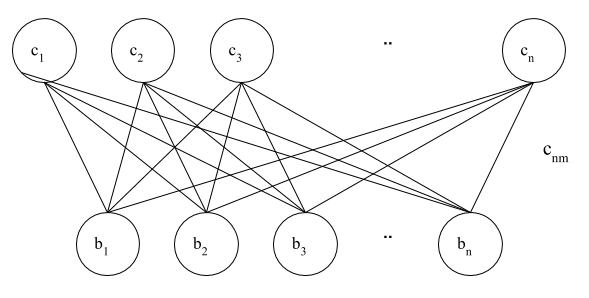
\includegraphics{Network_graph_of_RBM.png}}
	\caption{Network graph of RBM given n hidden units, and m visible units.}
	\label{fig:rbmexample}
\end{figure}

RBM defines a probability distribution, via the energy function, between each units’ weights and biases. This distribution is defined as
\begin{equation} \label{eq:1}
p(v, h) = \frac{e^{-E(v, h)}}{Z}
\end{equation}
\noindent where $Z$ is the partition function, and  $E(v, h)$ is the energy function defined as 
\begin{equation}\label{eq:2}
E(v, h) = \sum^V_{i=1} \sum^H_{j=1}  w_{ij} v_i h_j - \sum^V_{i=1}a_iv_i - \sum^H_{j=1}b_jh_j
\end{equation}
\noindent where the $v_i$ is the visible unit $i$, $h_j$ is the hidden unit $j$, $w_{ij}$ is the weight between $v_i$ and $h_j$, $a_i$ and $b_j$ are their biases. $V$ and $H$ represent the number of visible and hidden units, respectively. 
The distribution of the visible units’ weights and biases is defined as 
\begin{equation}\label{eq:3}
p(v) = \sum_H p(v, h) = \sum_H \frac{e ^ {-E(v, h)}}{Z}
\end{equation}

In RBMs, the units of the same layer are independent which do not have any connection with each other. In terms of probability, this means that the hidden variables are independent given the state of the visible variables and vice versa. Thus, the condition distributions of $p(h|v)$ and $p(v|h)$ are defined as
\begin{equation}\label{eq:4}
p(h_j = 1 | v) = \sigma\left( \sum^V_{i=1} w_{ij}v_i + b_j \right)
\end{equation}
\begin{equation}\label{eq:5}
p(v_i = 1 | h) = \sigma\left( \sum^H_{j=1} w_{ij}h_j + a_i \right)
\end{equation}
\noindent where $\sigma(x) = \frac{1}{1 + e^{-x}}$, the sigmoid function of x, the feature, element-wise.

In DBN’s pre-training, each RBM is trained individually, greedy layer-wise. The weights of each units’ connections, and each layer’s biases, are computed within this phase and saved for fine-tuning. This learning is repeated, from RBM to another, until all hidden layers are trained. This process can be expressed as follows 
\begin{equation}\label{eq:6}
p(h_j^{(l-1)} = 1 | v) = \sigma( \sum^V_{i=1} w_{ij}^{(l)}v_i^{(l)} + b_j^{(l-1)} )
\end{equation}
\noindent where $l$ corresponds to the current layer. 
The formulas and equations for RBM are based from the papers of \shortciteA{koesdwiady:2016, Fischer2014, zhang:2017}. 




\section{ParseHub}
ParseHub is a free web scraping tool that collects from any JavaScript or AJAX site. This web scraping tool can also export the collected data in CSV and JSON files. The tool also has the ability to cloud host which enables the data scraped to be saved through the cloud, and schedule a run to a future time. ParseHub can scrape from hundreds of pages depending on the pricing. The Free ParseHub may only collect 200 pages worth of data in under 40 minutes. It also can run 200 pages per run. Lastly, ParseHub retains data collected for 14 days.



\section{Performance Indices}
\subsection{RMSE and MAE}
% RMSE and MAE
To evaluate a model’s performance, many studies have employed using two of the most used performance indexes: the root mean squared error (RMSE) and the mean absolute error (MAE) \shortcite{chai2014RMSEorMAE}. The RMSE is used as a standard statistical system of measurement to calculate a model's performance, especially in air quality, meteorology, and climate research studies. It is defined using this function: 

\begin {equation}
r = \sqrt[]{\frac{1}{n}\sum_{i=1}^{n}(x_i - y_i)^2}
\end{equation}

\noindent where $n$ is the number of samples, $x_i$ and $y_i$ are the errors being observed at a certain $i$. On the other hand, MAE is a measure of the absolute difference between the errors. It is defined using this function: 

\begin {equation}
r = \frac{1}{n}\sum_{i=1}^{n}|x_i - y_i|
\end{equation}

\subsection{Sensitivity Analysis}
Sensitivity analysis is a study of how much the input variables clearly affect the outcome of a model \shortcite{saltelli2000}. It is also called the simulation analysis, wherein the results are predicted based on a range of input variables. Calculating the sensitivity that is dependent on time, we calculate the sensitivity relative to the initial parameters, inputs, or conditions in the model. 

The “time-dependent” sensitivities of output $Y$ relative to every input variable are “time-dependent” derivatives is given by the equation:

\begin{comment}

\begin{equation}
\frac{\partial a}{\partial b},
\qquad
\frac{\partial a}{\partial c}
\end{equation}

\end{comment}

\begin{equation}
\abs*{\frac{\partial Y}{\partial X_i}}_{X^0}
\end{equation}

\noindent where, $Y$ is the output and $X_i$ is the input factor. $X^0$ indicates that the derivative is taken at some fixed point in the space of the input. This shows that per input of the model, the ratio of its derivative with respect to its output is computed to get the sensitivity.

\begin{comment}
\noindent where, the $\partial a$ is the output and the $\partial b$ and $\partial c$ are the inputs of neural networks. This shows that per input of the model, the ratio of its derivative with respect to its output is computed to get the sensitivity.
\end{comment}

Several researchers have been applying sensitivity analysis to their models, particularly to the models which uses neural networks. In \shortciteA{hunter2000}, they applied sensitivity analysis of neural network inputs to their trauma survival prediction model to analyze the Trauma and Injury Severity Score (TRISS) variables used in their model. Their experiments on the variable’s sensitivity show that age is the most prominent variable in predicting survival. The researchers defined three approaches to sensitivity analysis. First is to introduce noise to every input variable and to observe its effects to the results. Second is to examine the derivatives of the weights of the input variables. Last is the proposed form of analysis based from the missing value problem approach. 

In \shortciteA{refenes1994}, they performed sensitivity analysis to evaluate their model on stock performance using neural networks. They used scatter plots to visually analyze the change in their network output (the likelihood of a sample being a target) with respect to the network input (stock factors). Based on their result, they were able to explain the predictive behavior of their neural network output by using sensitivity analysis. Furthermore, they were able to conclude that compared to regression models, their model can model the situation more convincingly.

